
\section{Definition of compensators}

\begin{frame}
	\frametitle{Lead Compensator vs Lag Compensator}
	\begin{block}{Schematical representation}
		\begin{figure}
			\centering
			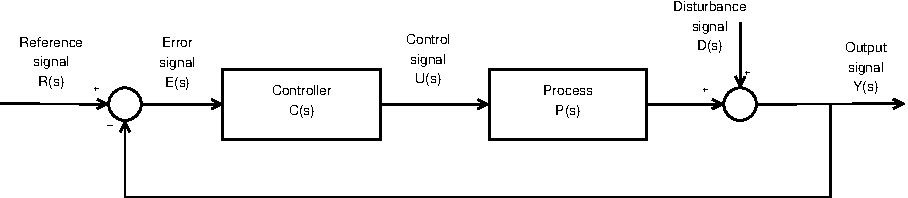
\includegraphics[width=1\linewidth]{Closed-Loop}
		\end{figure}
	\end{block}
	\begin{block}{Transfer functions}
		Lead compensator : 
		$C(s) = K.\frac{s + \frac{1}{\tau}}{s + \frac{1}{\alpha\tau}}$ with $0 \textless  \alpha  \textless  1$ \\
		Lag compensator : 
		$C(s) = K.\frac{s + \frac{1}{\tau}}{s + \frac{1}{\beta\tau}}$ with $\beta  \textgreater  1$
	\end{block}
\end{frame}

\begin{frame}
\frametitle{Lead Compensator vs Lag Compensator: zeros and poles}
\begin{block}{Transfer functions}
	Lead compensator : 
	$C(s) = K.\frac{s + \frac{1}{\tau}}{s + \frac{1}{\alpha\tau}}$ with $0 \textless  \alpha  \textless  1$ \\
	Lag compensator : 
	$C(s) = K.\frac{s + \frac{1}{\tau}}{s + \frac{1}{\beta\tau}}$ with $\beta  \textgreater  1$
\end{block}
\begin{block}{Zeros and poles}
	Zeros: $s = -\frac{1}{\tau}$ \\
	Poles: $s = -\frac{1}{\alpha\tau}$ or $s = -\frac{1}{\beta\tau}$ \\
	For lead compensators the pole lies more to the left in the complex plane than the zero and vice versa for lag compensators.
\end{block}
\end{frame}

\section{Lead compensators}

\begin{frame}
\frametitle{Lead compensators}
	\begin{block}{Transfer function}
		$C(s) = K.\frac{s + \frac{1}{\tau}}{s + \frac{1}{\alpha\tau}}$ with $0 \textless  \alpha  \textless  1$
	\end{block}
	\begin{block}{Bode Diagram}
		Example with K = 10 and $\alpha$ = 0.1 (see next slide) \\
		Magnitude of the lead compensator:
		\begin{itemize}
			\item becomes unity (= 0 dB) for small fequencies
			\item becomes 10 (= 20 dB) for high frequencies
		\end{itemize}
		$\Rightarrow$ Lead compensator is high-pass filter.
	\end{block}
\end{frame}

\begin{frame}
\frametitle{Lead compensators}
\begin{block}{Bode Diagram}
\begin{figure}
	\centering
	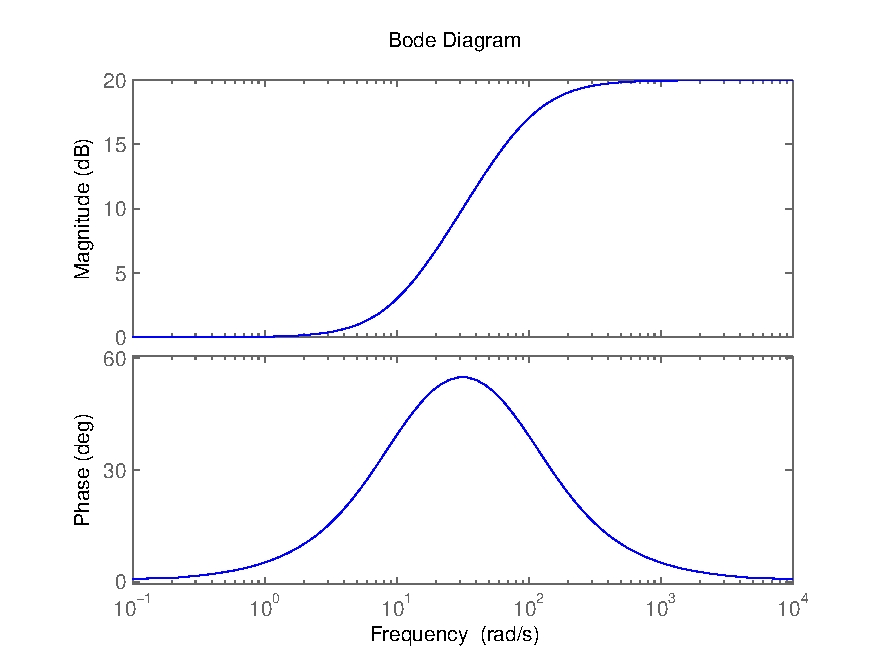
\includegraphics[width=0.7
	\linewidth]{bodeleadfilter2}
\end{figure}
\end{block}
\end{frame}

\begin{frame}
\frametitle{Lead compensators}
\begin{block}{Impact}
	\begin{itemize}
	\item Push the pole of the closed loop system to the left.
	\begin{itemize}
	\item Stabilisation of the system (see root locus)
	\item Increase response speed (lead compensator will stimulate some larger frequencies)
	\end{itemize}
	\item Increase of the phase margin: the phase of the lead compensator is positive for every frequency, and will hence only increase the phase.
	\item Thanks to the presence of a pole, the high frequencies (where most of the unwanted noise is located) are less amplified. Again, a lead compensator is a high-pass filter.
	
	\end{itemize}
\end{block}
\end{frame}

\begin{frame}
\frametitle{Lead compensators}
\begin{block}{Design with Bode plots}
	\begin{itemize}
		\item Design process: tuning of the phase margin, with as a surplus (because we will have one extra degree of freedom) the tuning of the steady state error.
		\item Compensate for the excessive phase lag that is a result of the components of P(s).
		\item Increase in phase at gain crossover frequency (GCF) if GCF is around pole and zero of the lead compensator.
		\item Gain is impacted by the lead compensator: the GCF of P(s).C(s) is not equal to the GCF of P(s).
		\item Required increase in phase gain: $\phi$
		\item K will be used to tune the steady state error.
	\end{itemize}		
\end{block}
\end{frame}	

\begin{frame}
	\frametitle{Lead Compensation Techniques Based on the Frequency-Response Approach}
	\begin{block}{Step 1}
		\begin{itemize}
			\item Remember the steady-state error for references of the shape: $\frac{At^n\epsilon(\tau)}{n!}$ with $\epsilon(t)$ the step function.
			\item Translate your steady-state requirement into another one:
			\begin{itemize}
				\item $K_p = \lim_{s \to 0} P(s)C(s)$ (n = 0, proportional)
				\item $K_v = \lim_{s \to 0} sP(s)C(s)$ (n = 1, linear)
				\item $K_a = \lim_{s \to 0} s^2P(s)C(s)$ (n = 2, accelerating)
				\item or another error constant
			\end{itemize}
			\item With this $K_p/K_v/K_a$ and $\lim_{s \to 0} P(s)$, we can determine $\lim_{s \to 0}C(s) = \lim_{s \to 0} K\frac{s + \frac{1}{\tau}}{s + \frac{1}{\alpha\tau}} = K\alpha$.
			\item Verify whether a proportional controller with gain $K\alpha$ would suffice.
		\end{itemize}
	\end{block}
\end{frame}

\begin{frame}
	\frametitle{Lead Compensation Techniques Based on the Frequency-Response Approach}
	\begin{block}{Step 2}
		Determine $\phi$, the amount with which you want to increase the PM; if the PM is OK, you don’t need a lead compensator; a proportional controller with gain $K\alpha$ suffices.
	\end{block}
	\begin{block}{Step 3}
		Add $5\,^{\circ}$, to get $\phi_m = \phi + 5\,^{\circ}$ (if $\phi_m > 60\,^{\circ}$, you will need more than one lead compensator). The addition of the lead compensator shifts the gain crossover frequency to the right and decreases the
		phase margin.
	\end{block}
\end{frame}

\begin{frame}	
	\frametitle{Lead Compensation Techniques Based on the Frequency-Response Approach}
	\begin{block}{Step 4}
		Determine $\alpha$ making use of the polar plot of 
		$\frac{\alpha.(j\omega\tau + 1)}{j\omega\alpha\tau + 1}$	
		\begin{figure}
			\centering
			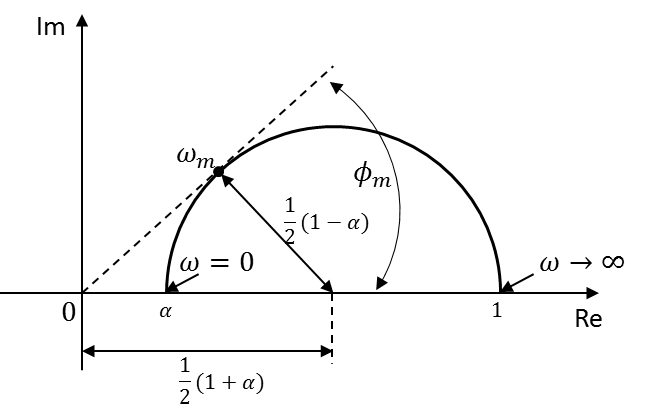
\includegraphics[width=0.4
			\linewidth]{leadcompalphabepalen}
		\end{figure}
		$\sin\phi_m = \frac{\frac{1}{2}.(1 - \alpha)}{\frac{1}{2}.(1 + \alpha)} = \frac{1 - \alpha}{1 + \alpha} \Rightarrow \alpha = \frac{1 - \sin\phi_m}{1 + \sin\phi_m}$ Usually, $\alpha \geqslant 0.05$. \\
		We know $\alpha$ and we know $K\alpha$ (step 1), so we can calculate K.
	\end{block}
\end{frame}

\begin{frame}
	\frametitle{Lead Compensation Techniques Based on the Frequency-Response Approach}
	\begin{block}{Step 5}
		Use the gain crossover frequency of P(s)C(s) as $\omega_m$: \\
		$\mid P(j\omega_m)C(j\omega_m) \mid = 1$ \\
		$\mid P(j\omega_m) \mid K \frac{\sqrt{\frac{1}{\alpha\tau^2} + \frac{1}{\tau^2}}}{\sqrt{\frac{1}{\alpha\tau^2} + \frac{1}{\alpha^2\tau^2}}} = \mid P(j\omega_m) \mid K \sqrt{\alpha} = 1$ \\
		$20\log \mid P(j\omega_m) \mid = -20\log (K\sqrt{\alpha})$ \\
		The value of the tangent point $\omega_m$ can be determined from P(s)'s Bode plot, because we know K and $\alpha$ from step 4.
	\end{block}
\end{frame}

\begin{frame}
	\frametitle{Lead compensators}
	\begin{block}{Step 6}
		\begin{figure}
			\centering
			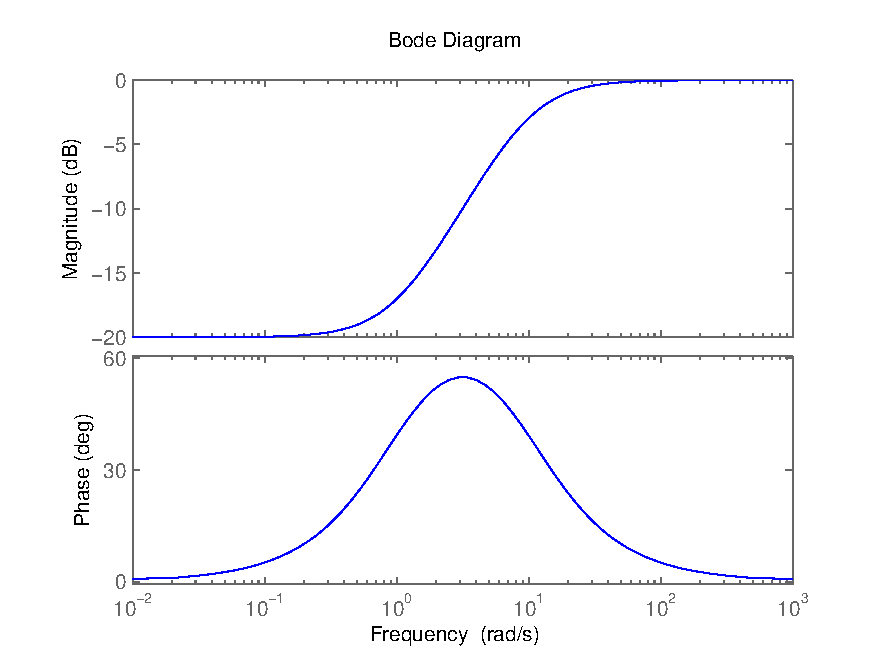
\includegraphics[width=0.5
			\linewidth]{bodelead}
		\end{figure}
		The tangent point $\omega_m$ is the geometric mean of the two corner frequencies, so
		$ \log \omega_m = \frac{1}{2}(\log \frac{1}{\tau} + \log \frac{1}{\alpha\tau})$ with $\tau = \frac{1}{\omega}$
		\\ $\Rightarrow \omega_m = \frac{1}{\sqrt{\alpha}\tau} \Rightarrow \tau = \frac{1}{\sqrt{\alpha}\omega_m}$. 
	\end{block}
\end{frame}

\begin{frame}
	\frametitle{Lead Compensation Techniques Based on the Frequency-Response Approach}
	\begin{block}{Step 7}
		Verify if the system behaves as desired.
		Check the gain margin for you to be sure it is satisfactory. If not, repeat the design process
		by modifying the pole-zero location of the compensator until a satisfactory result
		is obtained.
	\end{block}
\end{frame}

\begin{frame}
\frametitle{Example}
\begin{block}{Example}
	Given the system $P(s) = \frac{4}{s(s+2)}$. We want a phase margin of at least $50\,^{\circ}$ and a steady-state error for slope reference of maximal $\frac{A}{20}$.
	\begin{figure}
		\centering
		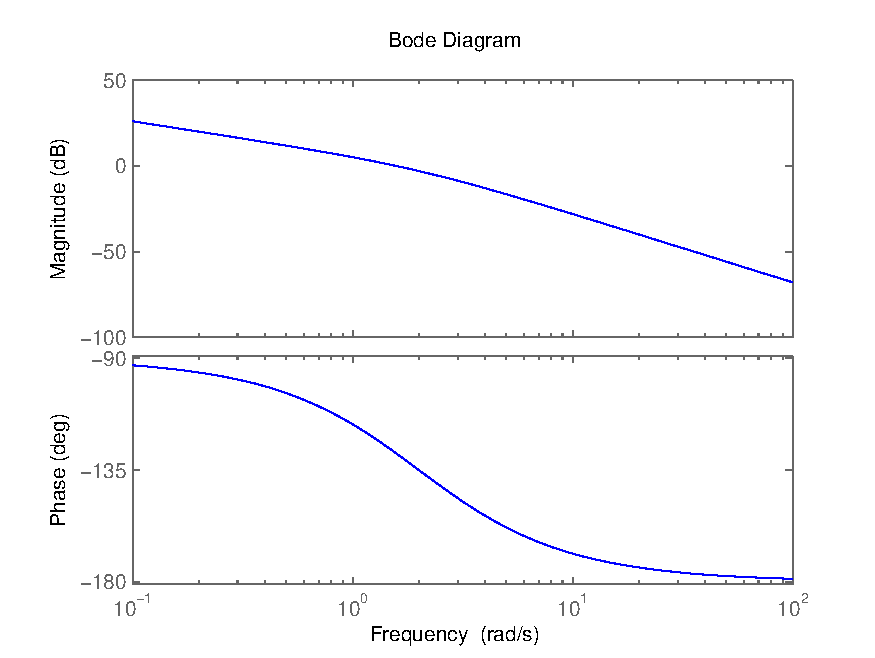
\includegraphics[width=0.5
		\linewidth]{bodeexamplelead}
	\end{figure}
\end{block}
\end{frame}

\begin{frame}
\frametitle{Example}
\begin{block}{Step 1}
\begin{itemize}	
\item Steady-state requirement: $K_v = \frac{20}{s}$ \\
So, $\lim_{s \to 0} sP(s)C(s) = \lim_{s \to 0} s\frac{4}{s(s+2)}K\alpha = 2K\alpha = 20$. \\
$\Rightarrow K\alpha = 10$
\item Would a proportional controller with gain $K\alpha$ suffice? We have a look at the Bode Diagram of $K\alpha P(s)$ (see next slide) \\
$\Rightarrow$ does not suffice! The phase margin is obviously smaller than $50\,^{\circ}$.
\end{itemize}
\end{block}
\end{frame}

\begin{frame}
\frametitle{Example}
\begin{block}{Bode Diagram $K\alpha P(s)$}
	\begin{figure}
		\centering
		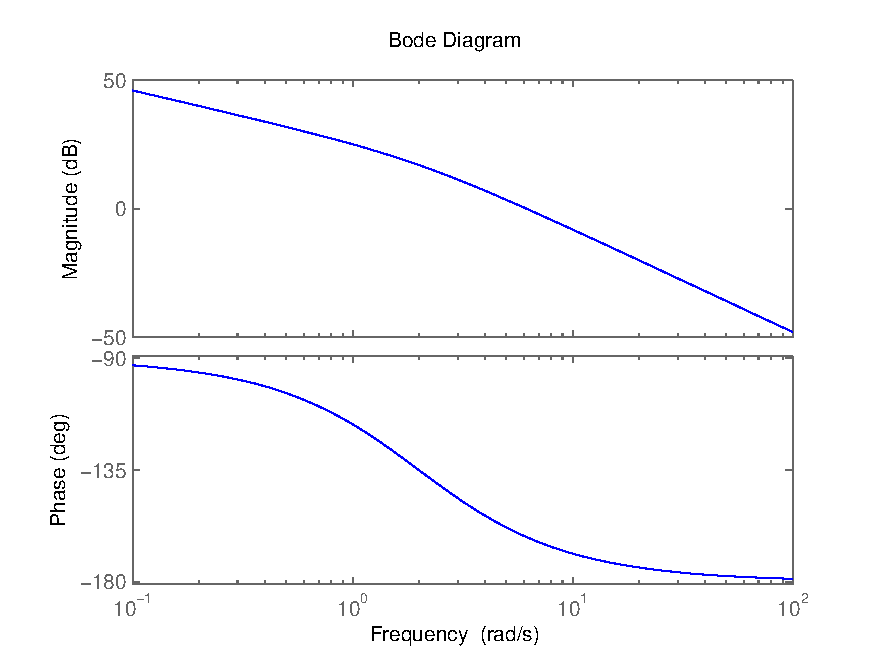
\includegraphics[width=0.6
		\linewidth]{bodeleadexamplestep1}
	\end{figure}
\end{block}
\end{frame}

\begin{frame}
\frametitle{Example}
\begin{block}{Step 2}
	\begin{itemize}
\item Phase margin of $K\alpha P(s) = 18\,^{\circ}$ (see last slide) \\
\item Calculation of phase margin without phase diagram: \\
We need the frequency where the magnitude is 0 dB. \\So, $20\log \mid K\alpha P(s) \mid = 0$
$\Rightarrow \mid K\alpha P(s) \mid = 1$
$\Rightarrow \mid P(s) \mid = 0.1$ \\
When substituting $s = j\omega$ and calculating the modulus of the complex number at the left side, the equation becomes: \\
$\frac{-4\omega}{\omega (4 + \omega^2)}^2 + \frac{-8}{\omega (4 + \omega^2)}^2 = 0.01$. \\
This equation has just one real positive solution: $\omega = 6.168$.\\
Now, you have the right frequency and you can calculate the phase margin exactly. 
\item We want a phase margin of at least $50\,^{\circ}$
$\Rightarrow \phi = 32\,^{\circ}$
\end{itemize}
\end{block}
\end{frame}

\begin{frame}
	\frametitle{Example}
\begin{block}{Step 3}
	$\phi_m = \phi + 5\,^{\circ} = 37\,^{\circ}$
\end{block}
	\begin{block}{Step 4}
		$\alpha = \frac{1 - \sin \phi_m}{1 + \sin \phi_m} = 0.24$ \\
		From step 1, we know that $K = \frac{\alpha}{10} = 42$
	\end{block}
	\begin{block}{Step 5}
		Find $\omega_m$, the frequency at which the gain is $-20\log(K\sqrt{\alpha})$ dB. 
		$GCF(P(s)K\sqrt{\alpha}) = GCF(P(s)C(s)) \Rightarrow \omega_m = 9 \frac{rad}{s}$ \\
		(see Bode Diagram next slide)
	\end{block}
\end{frame}

\begin{frame}
	\frametitle{Example}
	\begin{figure}
		\centering
		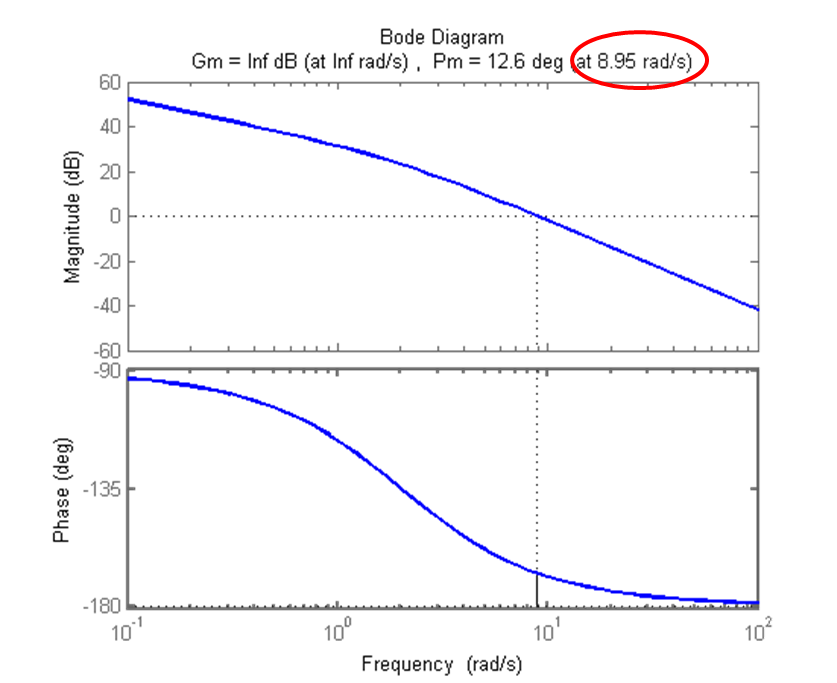
\includegraphics[width=0.7
		\linewidth]{exampleleadstep6}
	\end{figure}
\end{frame}

\begin{frame}
	\frametitle{Example}
	\begin{block}{Step 6}
		$\tau = \frac{1}{\omega_m\sqrt{\alpha}} = 0.23$
	\end{block}
	\begin{block}{Step 7}
	We verify whether or not our solution is correct. We ask the Bode Diagram of $K \frac{4}{s(s+2)} \frac{s+\frac{1}{\tau}}{s+\frac{1}{\alpha\tau}}$ with $\alpha$, $\tau$ and K the results of our calculations. (see next slide) \\
	We see that: 
	\begin{itemize}
		\item the phase margin is indeed more than $32\,^{\circ}$ 
		\item the new tangent point is indeed about $9\frac{rad}{s}$
	\end{itemize} 
	\end{block}
\end{frame}

\begin{frame}
\frametitle{Example}
\begin{figure}
	\centering
	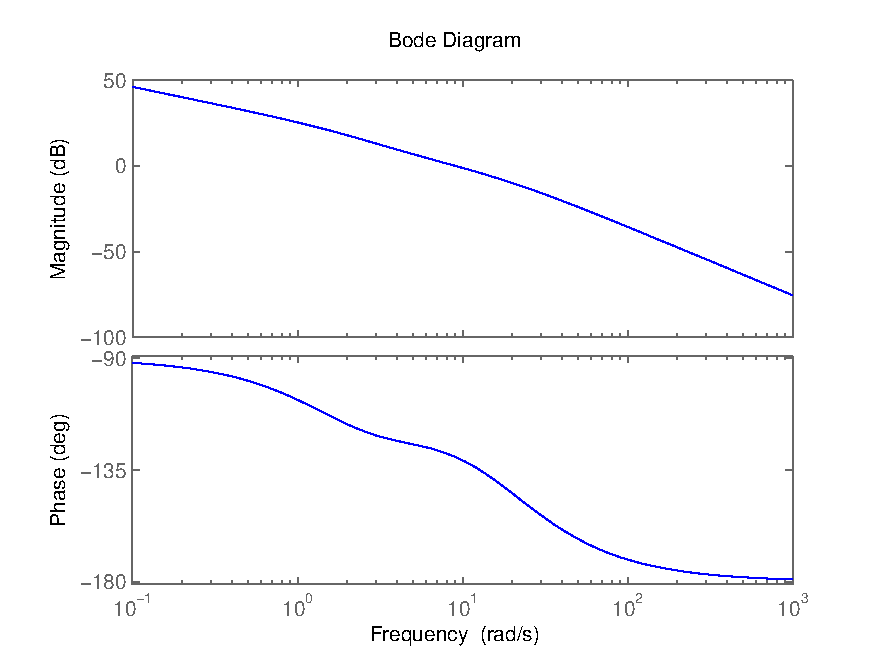
\includegraphics[width=0.7
	\linewidth]{bodesolutionexamplelead}
\end{figure}
\end{frame}

\begin{frame}
	\frametitle{Example}
	\begin{block}{Comparing compensated system vs non-compensated system}
	Blue: non-compensated system \\
	Green: compensated system
	\begin{figure}
		\centering
		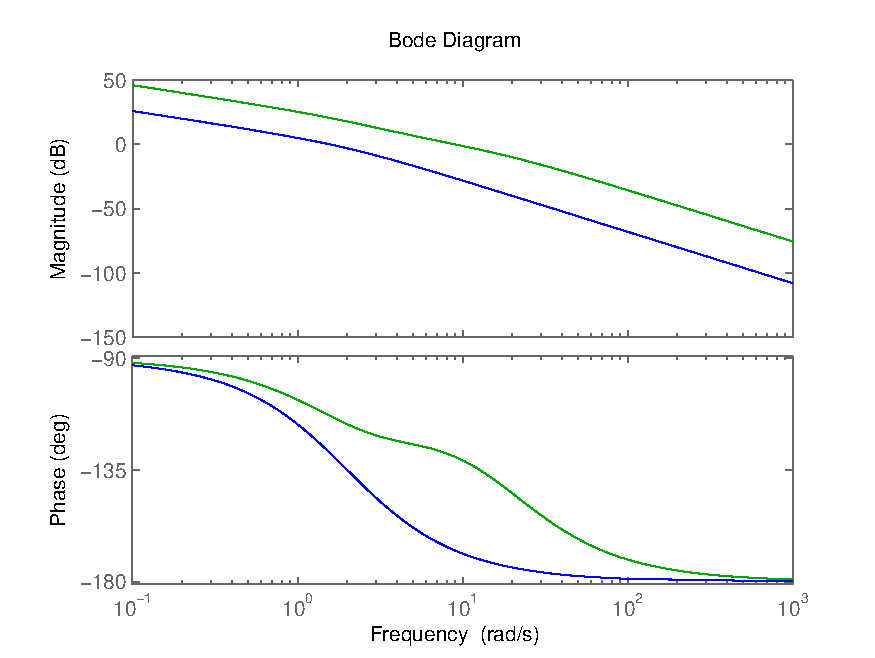
\includegraphics[width=0.5
		\linewidth]{bodesolutionexampleleadcomparing}
	\end{figure}
	\end{block}
\end{frame}

\begin{frame}
\frametitle{Summary lead compensators}
\begin{block}{Evaluation of impact}
\begin{itemize}
	\item Pushing the poles to the left: this is not directly visible here, but is linked to the increased band width.
	\item The increase in bandwidth (this is linked to the response speed) and the increase in the phase margin were apparent in the Bode plot of P(s)C(s).
	\item A (small) decrease in the steady-state error occurs, since we designed it as such. \\
	Why small? The steady-state error decreases when the DC gain gets larger, but a lead compensator’s impact on the gain is not really built to increase the DC gain, the shape of a lag compensator is much more fit for this.
\end{itemize}
\end{block}
\end{frame}

\begin{frame}
	\frametitle{Summary lead compensators}
	\begin{block}{Design with root locus}
	Design lead compensators with root locus for time-domain quantities  - use dominant pole locations to fulfill overshoot, rise time, settling time, damping ratio and other requirements.
	\end{block}
\end{frame}

\section{Lag compensators}

\begin{frame}
	\frametitle{Lag compensators}
	\begin{block}{Transfer function}
		$C(s) = K.\frac{s + \frac{1}{\tau}}{s + \frac{1}{\beta\tau}}$ with $\beta  \textgreater  1$
	\end{block}
	\begin{block}{Bode Diagram}
		Example with K = 1 and $\beta$ = 10 (see next slide) \\ 
		Magnitude of the lag compensator: 
		\begin{itemize}
			\item becomes 10 (= 20 dB) for small frequencies
			\item becomes unity (= 0 dB) for high frequencies
		\end{itemize}
		$\Rightarrow$ Lag compensator is low-pass filter.
		
	\end{block}
\end{frame}

\begin{frame}
\frametitle{Lag compensators}
\begin{block}{Bode Diagram of example}
	\begin{figure}
		\centering
		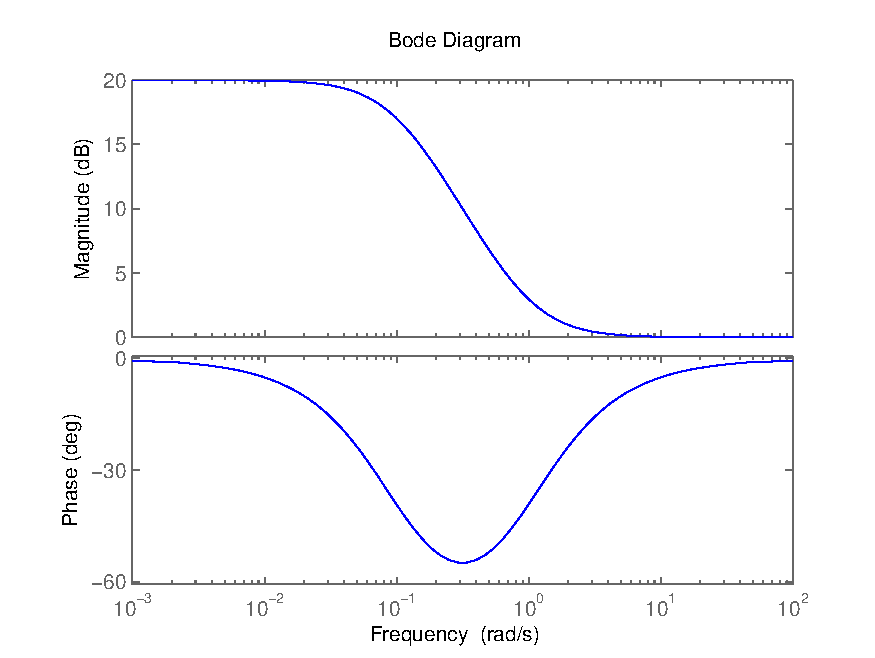
\includegraphics[width=0.5
		\linewidth]{bodelagislowpass}
	\end{figure}
\end{block}
\end{frame}

\begin{frame}
\frametitle{Lag compensators}
\begin{block}{Impact of lag compensators: Bode Diagram}
	Blue: non-compensated system \\
	Green: compensated system
	\begin{figure}
		\centering
		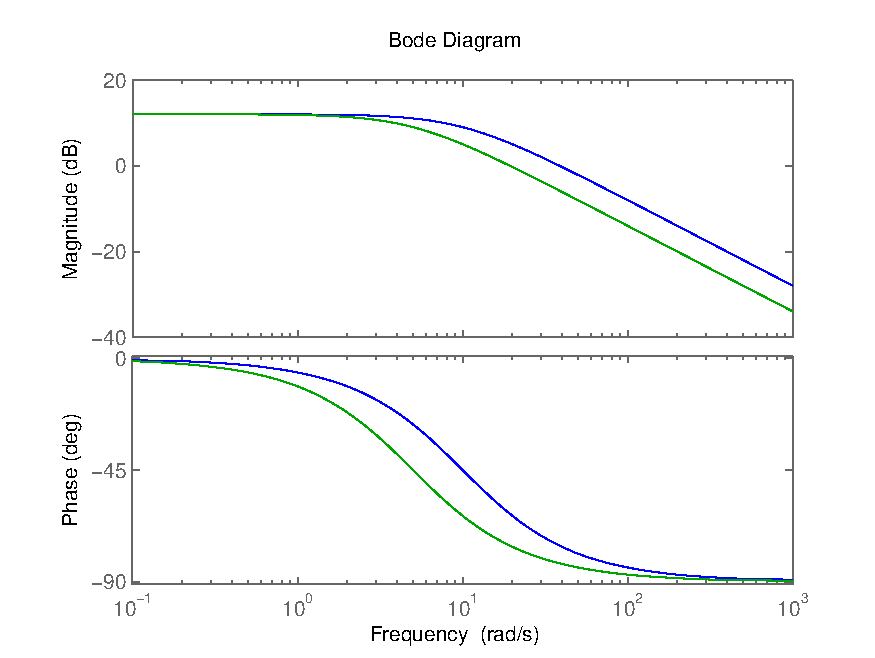
\includegraphics[width=0.5
		\linewidth]{bodelagimpact}
	\end{figure}
\end{block}
\end{frame}

\begin{frame}
	\frametitle{Lag compensators}
	\begin{block}{Impact of lag compensators: Bode Diagram}
	\begin{itemize}
		\item Lead compensators: increase the stability and tune the steady-state error by increasing the phase at the crossover frequency.
		\item Impact lag compensator = lead compensator, but different approach!
		By decreasing the gain, the gain crossover frequency comes down to a frequency at which the corresponding phase is higher.
		
	\end{itemize}
	\end{block}
\end{frame}

\begin{frame}
	\frametitle{Lag compensators}
	\begin{block}{Impact of lag compensators}
		Large difference between lead and lag: their effect on the bandwidth of the system and hence on its speed of response.
		\begin{itemize}
			\item A lead compensator increases the bandwidth/speed of response 
			\begin{itemize} 
			\item good if you want the system to react fast
			\end{itemize}
			\item A lag compensator decreases the bandwidth/speed of response 
			\begin{itemize}
			\item good if your model is bad at high frequencies
			\item good to reduce the impact of (mostly high-frequency) noise 
			\end{itemize}
		\end{itemize}
	\end{block}
\end{frame}

\begin{frame}
\frametitle{Lag compensators}
\begin{block}{Design with Bode plots}
We have three degrees of freedom:
\begin{itemize}
	\item one to have a sufficient drop in gain
	\item one to push the drop in the phase to lower frequencies (that way we can use $\measuredangle P(s)$ as an approximation of $\measuredangle P(s)C(s)$ reliably to some extent
	\item one to tune the steady-state error
\end{itemize}
		
\end{block}
\end{frame}

\begin{frame}
	\frametitle{Lag compensators}
	\begin{block}{Design with Bode plots}
		\begin{itemize}
		\item Increase of phase margin $\Rightarrow$ decrease of the magnitude at some higher frequencies 
		\item Decrease of the steady state error $\Rightarrow$ increase of the magnitude at DC
		\end{itemize}
		A lag compensator can realize both conditions.
		\begin{itemize}
			\item At DC value, the gain becomes: $\lim_{s \to 0} K\frac{s + \frac{1}{\tau}}{s + \frac{1}{\beta\tau}} = K\beta$
			\item At high frequencies, the gain becomes:
			$\lim_{s \to \infty} K\frac{s + \frac{1}{\tau}}{s + \frac{1}{\beta\tau}} = K$ 
		\end{itemize}
	\end{block}
\end{frame}

\begin{frame}
	\frametitle{Lag compensators}
	\begin{block}{Design with Bode plots}
	K has to be such that the drop in magnitude is sufficient, the value of $\beta$ has make the steady-state error decrease enough and the value of $\tau$ has to be such that the transfer between from $K\beta$ to $\tau$ occurs at the right frequency.
	\begin{figure}
		\centering
		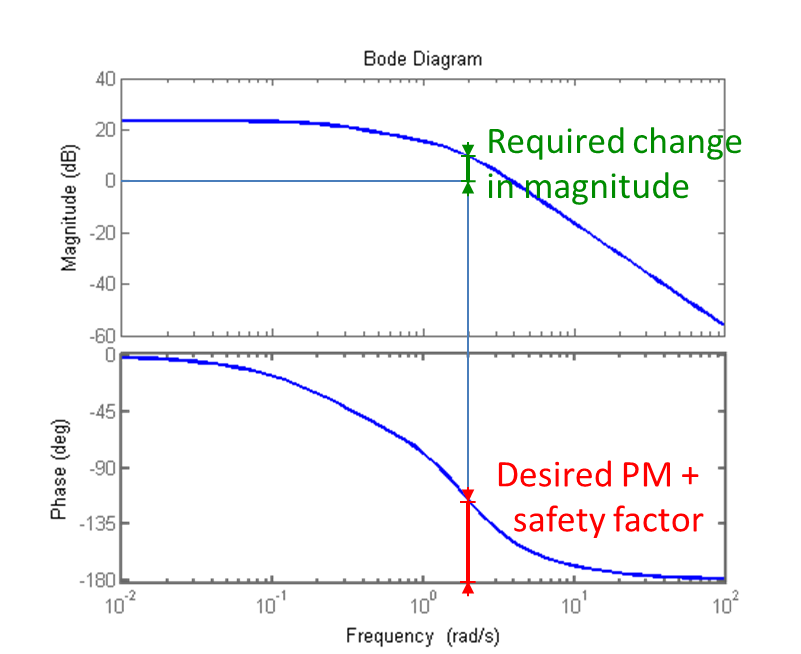
\includegraphics[width=0.45
		\linewidth]{determinationKLagcompensator}
	\end{figure}
	\end{block}
\end{frame}

\begin{frame}
\frametitle{Lag Compensation Techniques Based on the Frequency-Response Approach}
\begin{block}{Step 1}
	\begin{itemize}
	\item Determine $K\beta$ in a similar way as we found $K\alpha$ for the lead compensator.
	\item Translate your steady-state requirement into a requirement on:
	\begin{itemize}
		\item $K_p = \lim_{s \to 0} P(s)C(s)$
		\item $K_v = \lim_{s \to 0} sP(s)C(s)$
		\item $K_a = \lim_{s \to 0} s^2P(s)C(s)$
		\item or another error constant
	\end{itemize}
	\item With this $K_p/K_v/K_a$ and $\lim_{s \to 0} P(s)$, we can determine $\lim_{s \to 0}C(s) = K\beta$.
	\item Verify whether a proportional controller with gain $K\beta$ would suffice.
	\end{itemize}
\end{block}
\end{frame}

\begin{frame}
\frametitle{Lag Compensation Techniques Based on the Frequency-Response Approach}
\begin{block}{Step 2}
	\begin{itemize}
	\item Take the zero one decade smaller than the frequency ($\omega$) at which P(s) had the desired phase ($-180\,^{\circ}$ + the desired phase margin + a safety factor of $10\,^{\circ}$). The addition of $10\,^{\circ}$ compensates for the phase lag of the lag compensator.
	\item Verify the effect of a single zero at a frequency one decade smaller than $\omega$.
	\begin{itemize}
		\item The drop in magnitude is as good as complete.
		\item The drop in phase cannot be more than $-5.7\,^{\circ}$.
	\end{itemize}
	\item Compute $\tau = \frac{10}{\omega}$. $\tau$ has to be large enough such that the magnitude is almost entirely dropped, and the phase drop has almost disappeared.
	\end{itemize}
\end{block}
\end{frame}

\begin{frame}
\frametitle{Lag Compensation Techniques Based on the Frequency-Response Approach}
\begin{block}{Step 3}
	\begin{itemize}
	\item	Determine K from the Bode plot. \\
		How to do this?
		Find the frequency ($\omega$) with desired phase margin (+ safety factor), then find the magnitude at that frequency; which is equal to the required change in magnitude (= Q). \\
		$\Rightarrow$ $K = \frac{1}{Q}$ \\
		\item Safety factor about $10\,^{\circ}$
		\begin{itemize}
			\item the drop in magnitude will not be complete (this is very marginal)
			\item the lag compensator influences the phase plot
		\end{itemize}
	\end{itemize}
\end{block}
\end{frame}

\begin{frame}
\frametitle{Lag Compensation Techniques Based on the Frequency-Response Approach}
\begin{block}{Step 4}
	We just have calculated K (step 3) and we know $K\beta$ (step 1), so it's possible to determine $\beta$.
\end{block}
\begin{block}{Step 5}
	Verify the behavior of the resulting system.
\end{block}
\end{frame}

\begin{frame}
\frametitle{Example}
\begin{block}{Example}
Given the system $P(s) = \frac{1}{s(s+1)(s+2)}$. The system has a PM of $53.4\,^{\circ}$ at a frequency of $0.446\frac{rad}{s}$ and a GM of $15.6 dB$ at a frequency of $1.41\frac{rad}{s}$.
We want that a ramp input $A\epsilon(t)$ results in a steady-state error of at most $\frac{A}{5}$, or $K_v =\frac{5}{s}$ and a PM of at least $40\,^{\circ}$.
\begin{figure}
	\centering
	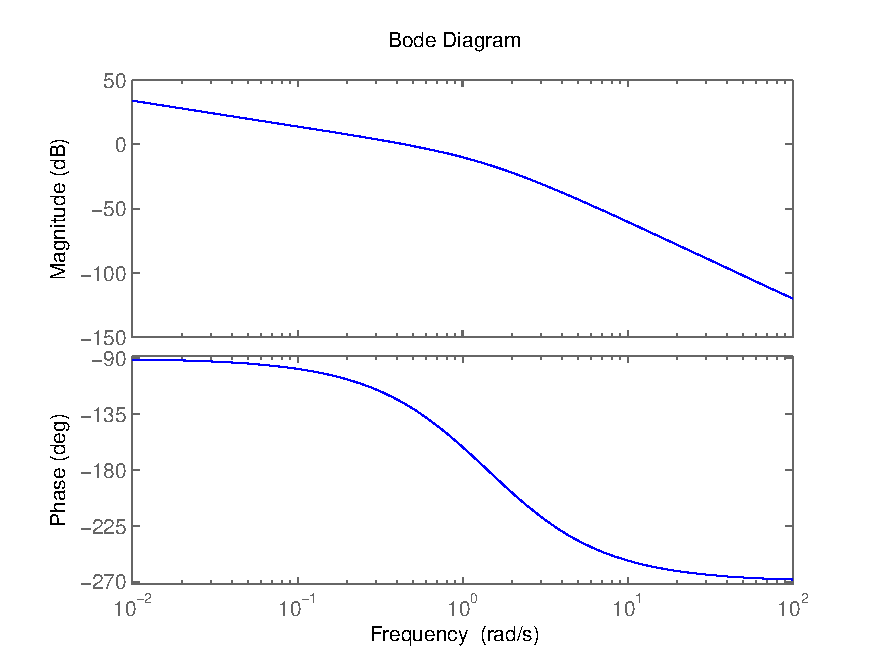
\includegraphics[width=0.5
	\linewidth]{bodeexamplelag}
\end{figure}
\end{block}
\end{frame}

\begin{frame}
\frametitle{Example}
\begin{block}{Step 1}
	\begin{itemize}
	\item Steady-state requirement: $K_v = \frac{5}{s}$ \\
	$\Rightarrow \lim_{s \to 0} sP(s)C(s) = \frac{1}{2}\lim_{s \to 0} C(s) = \frac{5}{s} \Rightarrow K\beta = 10$
	\item Would a proportional controller with gain $K\beta$ suffice? To answer this, we must have a look at the Bode plot of $K\beta P(s)$ (see next slide). \\
	$\Rightarrow$ Does not suffice! Adding a gain of $10 = 20 dB$ to get the right steady-state error, the phase gain would become negative. In other words, at the frequency where the magnitude of $K\beta P(s)$ equals 0 dB, the phase is less than $-180\,^{\circ}$ which means the system would become unstable.
	\end{itemize}
\end{block}
\end{frame}

\begin{frame}
\frametitle{Example}
\begin{block}{Step 1 continued}
\begin{figure}
	\centering
	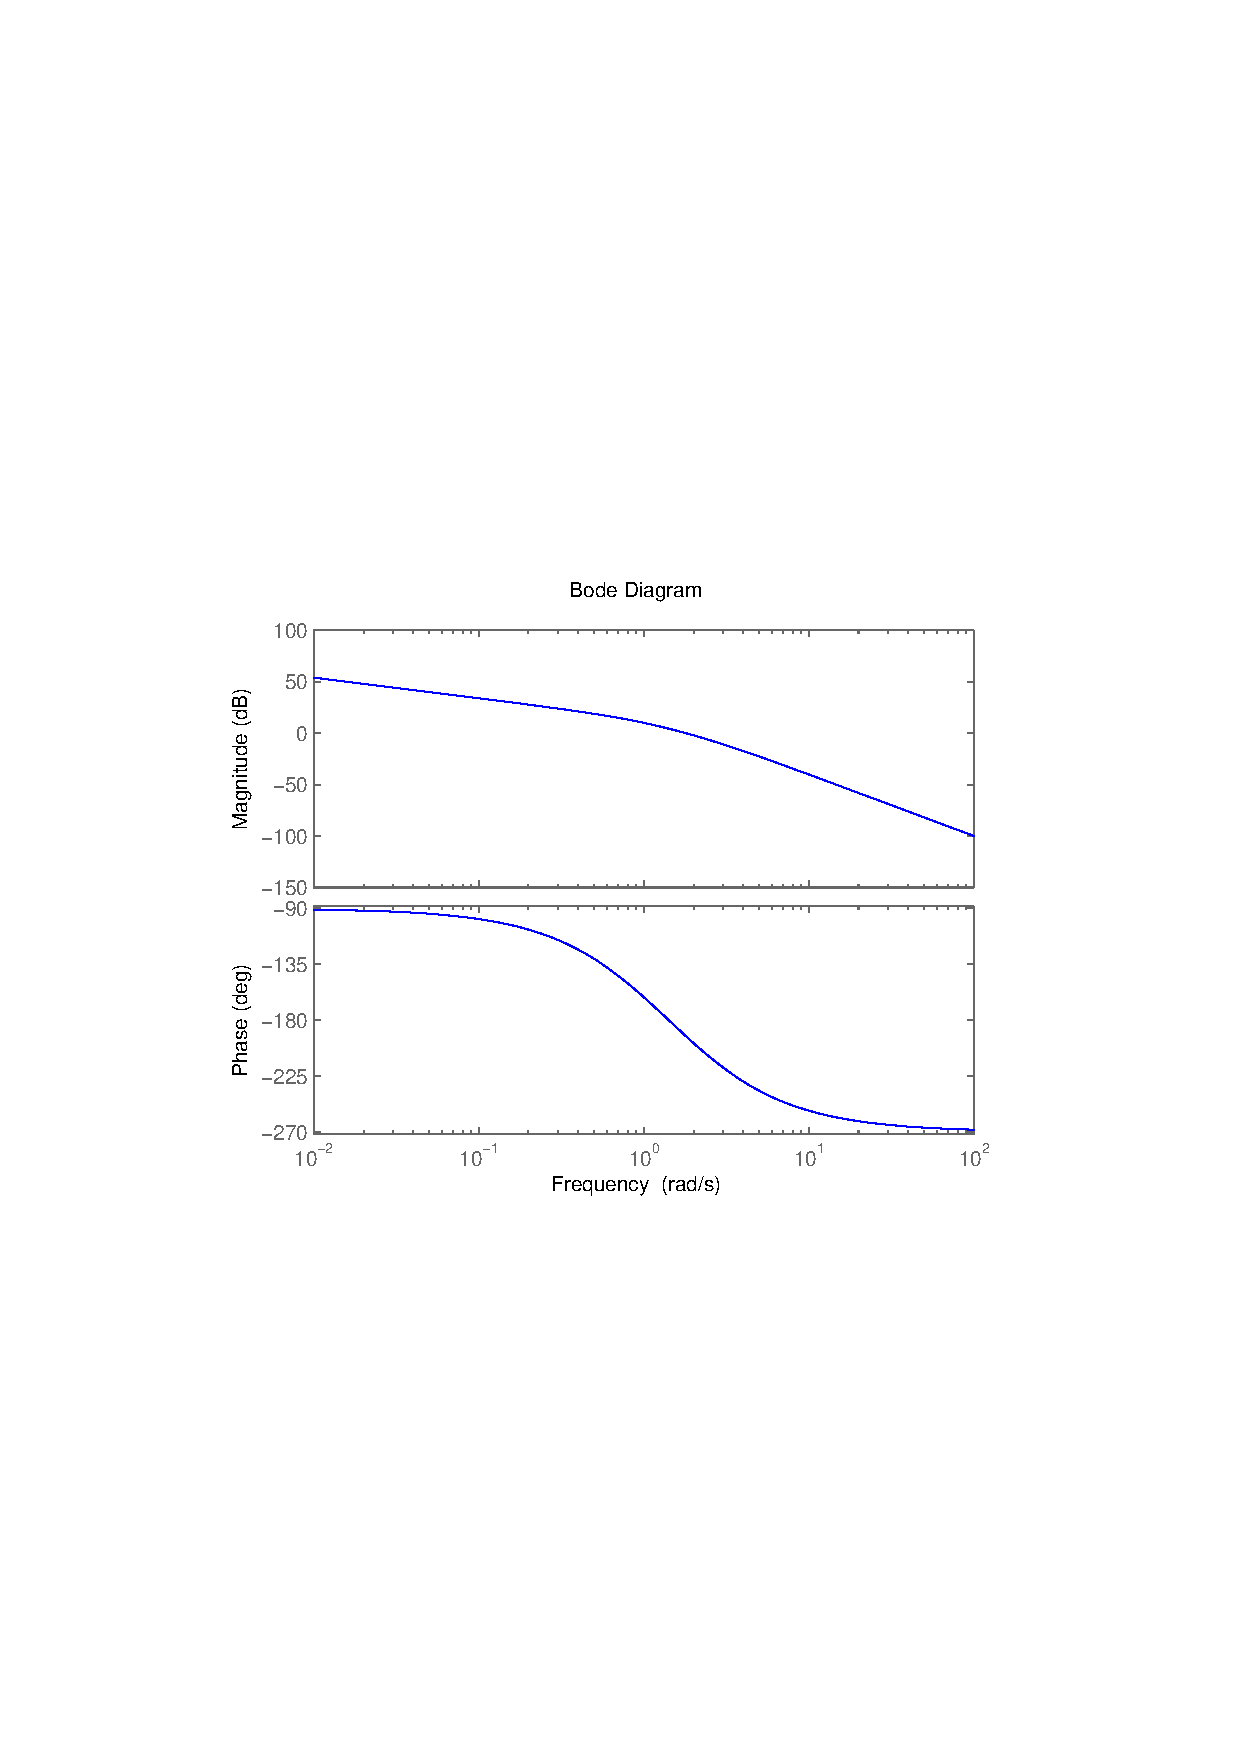
\includegraphics[width=0.5
	\linewidth]{bodeexamplelagpropnotgood}
\end{figure}	
\end{block}
\end{frame}

\begin{frame}
\frametitle{Example}
\begin{block}{Step 2}
\begin{figure}
	\centering
	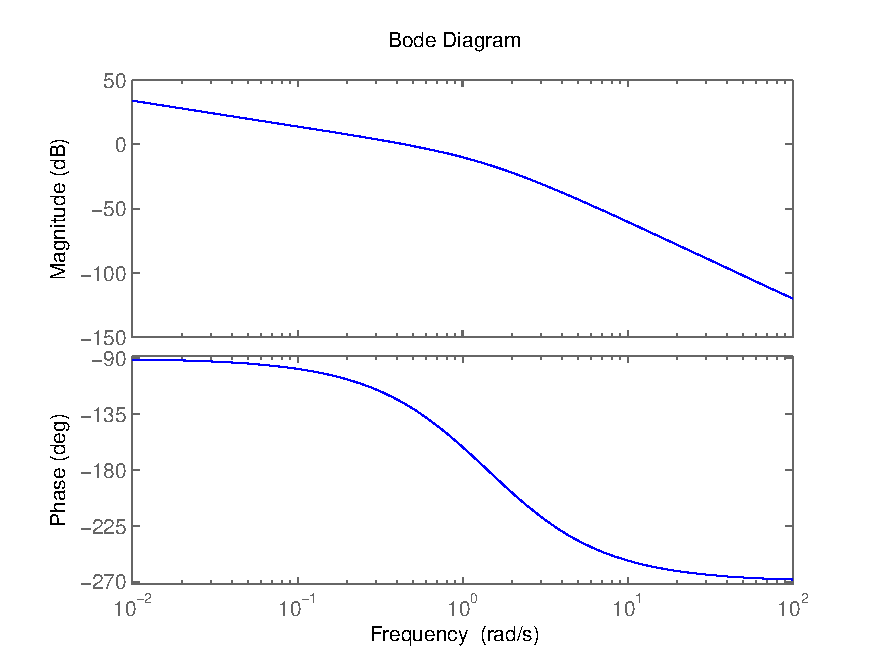
\includegraphics[width=0.5
	\linewidth]{bodeexamplelag}
\end{figure}
Determine required phase \\ $phase = -180\,^{\circ} + 40\,^{\circ} + 10\,^{\circ} = -130\,^{\circ}$ \\ At a phase of $-130\,^{\circ}$, $\omega = 0.5 \frac{rad}{s}$ $\Rightarrow \tau = \frac{10}{0.5} = 20$
\end{block}
\end{frame}

\begin{frame}
\frametitle{Example}
\begin{block}{Step 2 continued}
Verify the effect of a single zero at a frequency one decade smaller than $\omega$.
\begin{figure}
	\centering
	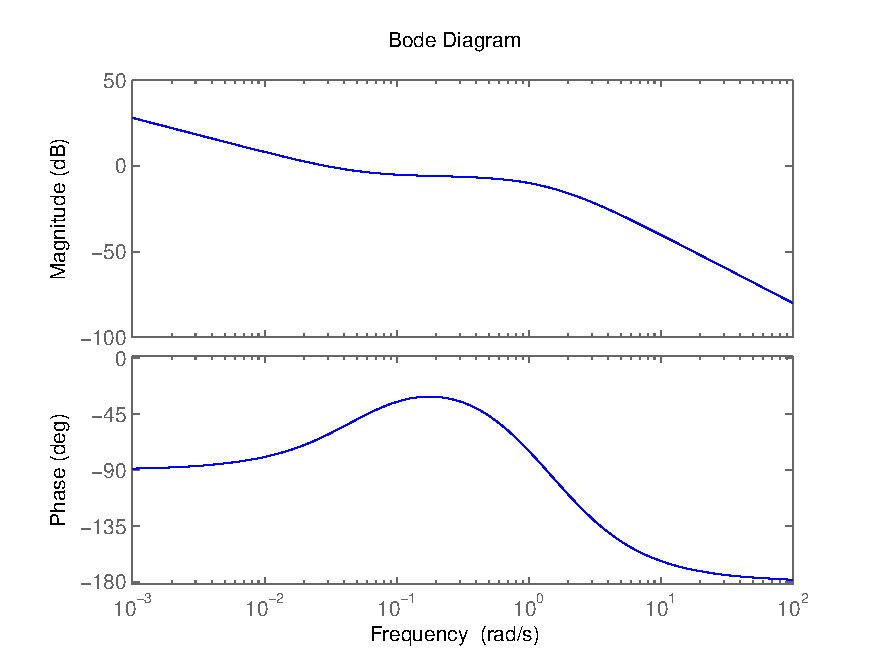
\includegraphics[width=0.5
	\linewidth]{bodeexamplelagstep2continued}
\end{figure}
\end{block}
\end{frame}

\begin{frame}
\frametitle{Example}
\begin{block}{Step 3}
At $\omega = 0.5 \frac{rad}{s}$, the magnitude equals 0 dB = 1, so Q = 1. \\
$K = \frac{1}{Q} = 1$
\begin{figure}
	\centering
	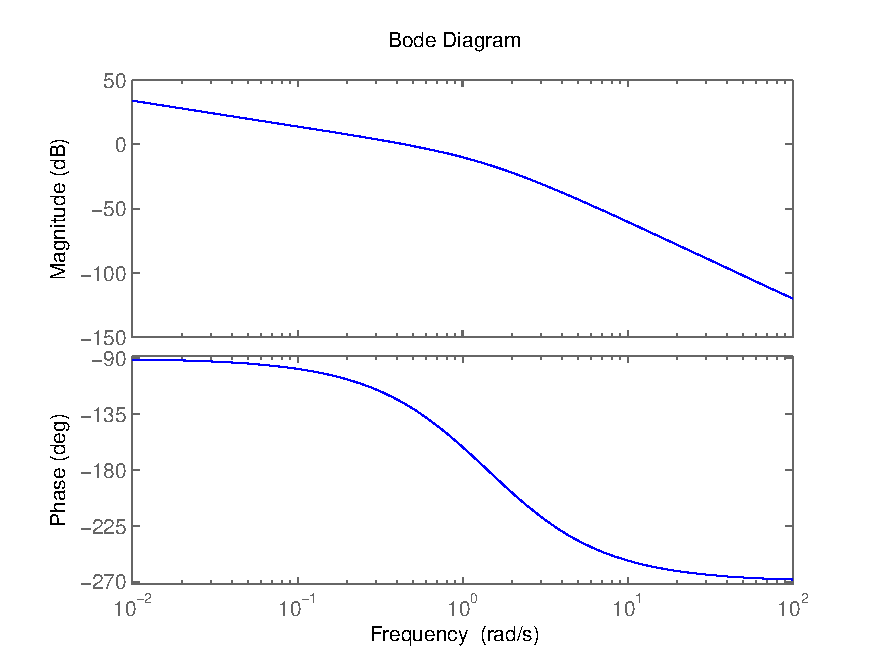
\includegraphics[width=0.5
	\linewidth]{bodeexamplelag}
\end{figure}
\end{block}
\end{frame}

\begin{frame}
\frametitle{Example}
\begin{block}{Step 4}
From the results of step 1 and step 3, we find $\beta = 10$.
\end{block}
\begin{block}{Step 5}
We find $C(s) = \frac{s + 0.05}{s + 0.05}$. \\ We verify the behavior of $P(s)C(s) = \frac{1}{s(s+1)(s+2)}\frac{s + 0.05}{s + 0.05}$ on its Bode Diagram (see next slide). \\
The phase margin is indeed greater than $40\,^{\circ}$.
\end{block}
\end{frame}

\begin{frame}
\frametitle{Example}
\begin{block}{Step 5 continued}
\begin{figure}
	\centering
	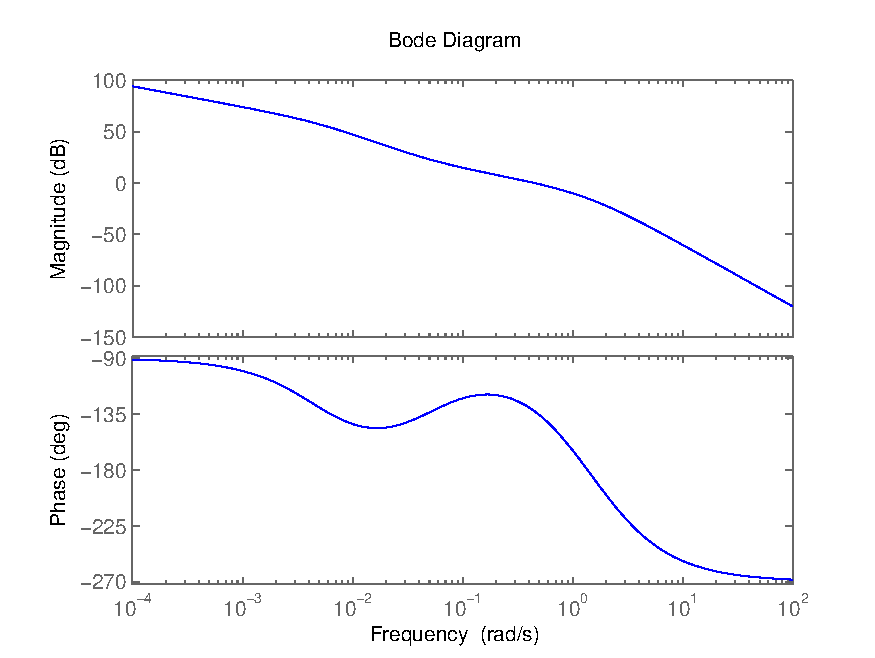
\includegraphics[width=0.5
	\linewidth]{bodeexamplelagstep5}
\end{figure}
\end{block}
\end{frame}

\begin{frame}
\frametitle{Example}
\begin{block}{Comparing compensated system vs non-compensated system}
Blue: non-compensated system \\
Green: compensated system
\begin{figure}
	\centering
	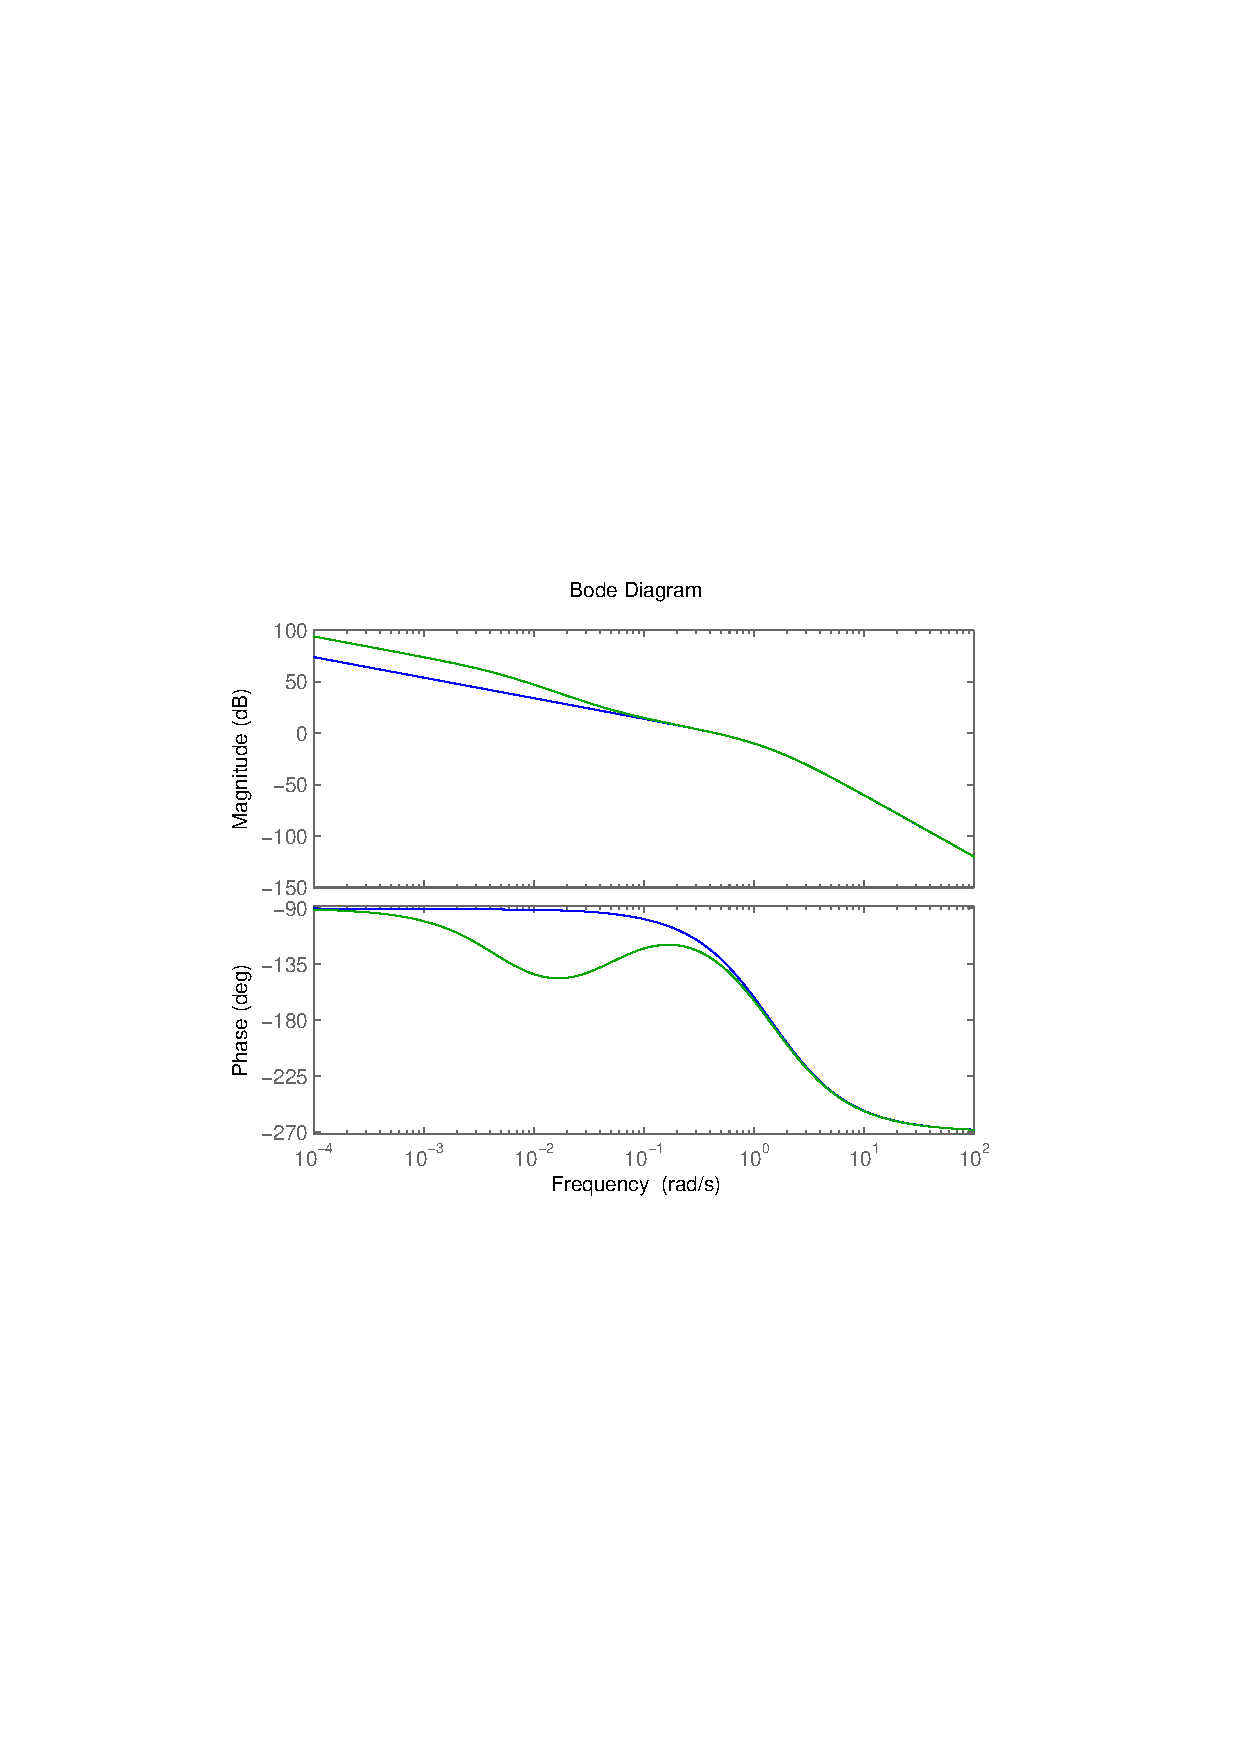
\includegraphics[width=0.5
	\linewidth]{bodeexamplelagcomparing}
\end{figure}
\end{block}
\end{frame}

\begin{frame}
\frametitle{Summary lead compensators}
\begin{block}{Goal}
	\begin{itemize}
\item To decrease the magnitude in order to shift the gain crossover frequency to a frequency with a larger phase margin; the extra degree of freedom is then used to tune the steady-state error.
\item In this example: lag compensator to tune the steady-state error with a minimal impact on the phase margin. \\
So this time we used a lag compensator to increase the DC gain but leave the gain at higher frequencies unaltered.
\end{itemize}
\end{block}
\end{frame}

\begin{frame}
\frametitle{Summary lead compensators}
\begin{block}{Impact, using root locus}
\begin{itemize}
\item We can use lag compensators to reduce the steady-state error significantly but with a marginal impact on (the relevant part of) the root locus.
\item On top of that, we still have one degree of freedom that allows us to pick any position on that root locus!
\item This is useful if the desired closed loop poles are already on the root locus, but if a proportional controller would give a too large steady-state error.
\end{itemize}
\end{block}
\end{frame}


\section{Lag-lead compensators}

\begin{frame}
\frametitle{Lag-lead compensators}
\begin{block}{Introduction}
	In some cases you would want to combine the effects of a lag and a lead compensator:
	\begin{itemize}
		\item Frequency domain: \\
		In most cases a lead compensator is more fit to increase the phase margin and a lag compensator is better at 	decreasing the steady-state error.
		\item Time domain: \\
		You might want to adapt the root locus with a lead compensator, and decrease the steady-state error while leaving the new root locus unaltered with a lag 	compensator.	
	\end{itemize}
\end{block}
\end{frame}

\begin{frame}
\frametitle{Lag-lead compensators}
\begin{block}{Transfer function}
	$C(s) = K\frac{s + \frac{1}{\tau_1}}{s + \frac{1}{\alpha\tau_1}}\frac{s + \frac{1}{\tau_2}}{s + \frac{1}{\beta\tau_2}}$ with $\beta \textgreater 1$, $0 \textless \alpha \textless 1$, $\tau_1 \textless \tau_2$ \\
	Usually, we take $\beta$ = $\frac{1}{\alpha}$, but that's not necessary. \\
	\begin{itemize}
	\item The term $\frac{s + \frac{1}{\tau_1}}{s + \frac{1}{\alpha\tau_1}}$ produces the effect of the lead network.
	\item The term $\frac{s + \frac{1}{\tau_2}}{s + \frac{1}{\beta\tau_2}}$ produces the effect of the lag network.
	\item Zeros: $\frac{1}{\tau_1}$ and $\frac{1}{\tau_2}$
	\item Poles: $\frac{1}{\alpha \tau_1}$ and $\frac{1}{\beta \tau_2}$
	\end{itemize}
\end{block}

\end{frame}

\begin{frame}
\frametitle{Lag-lead compensators}
\begin{block}{Bode Diagram}
Example with K = 10, $\alpha$ = 0.1, $\beta$ = 10, $\tau_1$ = 0.01, $\tau_2$ = 10 (see next slide) \\
Magnitude of lag-lead compensator:
\begin{itemize}
\item becomes 10 (= 20 dB) at low frequencies
\item becomes unity (= 0 dB) at frequencies of about $1 \frac{rad}{s}$ to $10 \frac{rad}{s}$
\item becomes 10 (= 20 dB) at high frequencies
\end{itemize}
$\Rightarrow$ Lag-lead compensator is a band stop filter \\
Explanation: $\beta \tau_2 \textgreater \tau_2 \textgreater \tau_1 \textgreater \alpha \tau_1$ \\
$\Rightarrow \frac{1}{\beta \tau_2} \textless \frac{1}{\tau_2} \textless \frac{1}{\tau_1} \textless \frac{1}{\alpha \tau_1}$ \\
$\Rightarrow$ $pole_1 \textless zero_1 \textless zero_2 \textless pole_2$
\end{block}
\end{frame}

\begin{frame}
\frametitle{Lag-lead compensators}
\begin{block}{Bode diagram}
\begin{figure}
	\centering
	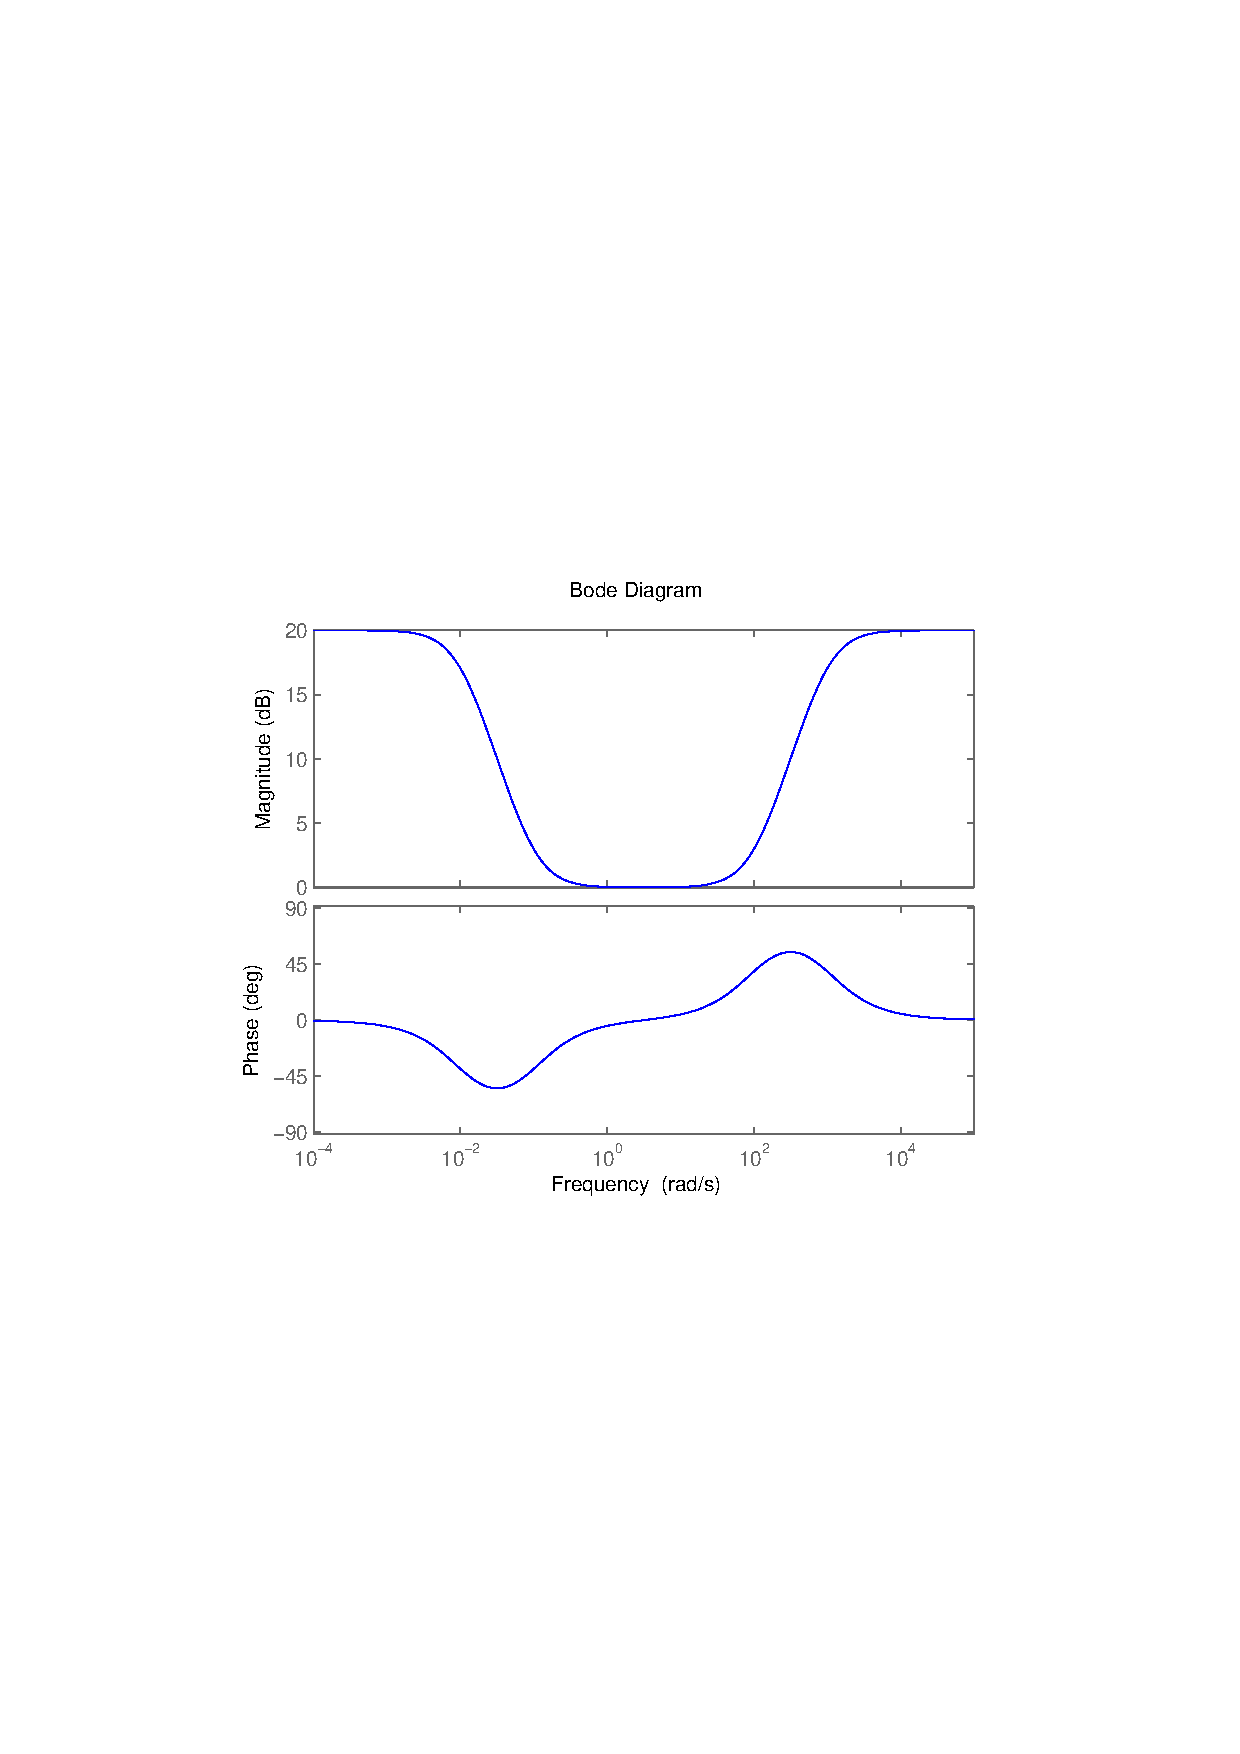
\includegraphics[width=0.5
	\linewidth]{laglead}
\end{figure}	
\end{block}
\end{frame}

\begin{frame}
\frametitle{Lag-lead compensators}	\begin{block}{Bode diagram}
	Both the good properties of a lag and a lead compensator are used:
	\begin{itemize}
	\item At low frequencies, the lag compensator is meant to decrease the steady-state error (see amplitude diagram).
	\item At middle frequenties, the lag compensator is meant to increase the phase margin (see amplitude diagram).
	\item At high frequencies, the lead compensator is meant to increase the phase margin (see phase diagram). 
	\end{itemize}
\end{block}
\end{frame}

\begin{frame}
\frametitle{Lag-lead compensators}
\begin{block}{Bode Diagram}
	Define $\omega_l$ as the frequency at which the phase angle is zero. For any frequency less than $\omega_l$, the compensator behaves as a lag compensator. For any frequency greater than $\omega_l$, the compensator behaves as a lead compensator. \\
	It can be proved that $\omega_l = \sqrt{\frac{1}{\tau_1 \tau_2}}$
	Prove: pag 649 in Ogata. Necessary?
\end{block}
\end{frame}

\begin{frame}
\frametitle{Lag-lead compensators}
\begin{block}{Disadvantage}
	The disadvantage of a lag-lead compensator over a lag compensator or a lead compensator is its increased complexity, and hence cost (the same way a lag or lead compensator is more complex/costly than a proportional controller).
\end{block}
\end{frame}

\section{Comparison lead, lag and lag-lead compensators}

\begin{frame}
\frametitle{Comparison lead, lag and lag-lead compensators}
\begin{block}{Method}
\begin{itemize}
\item Lead compensation achieves the desired result through the merits of its phaselead
contribution.
\item Lag compensation accomplishes the result through the merits of its attenuation property at high frequencies.
\end{itemize}
\end{block}
\end{frame}

\begin{frame}
\frametitle{Comparison lead, lag and lag-lead compensators}
\begin{block}{Band width}
Lead compensators are commonly used for improving stability margins and yields a higher gain crossover frequency than is possible with lag compensation. The higher gain crossover frequency means a larger bandwidth.
\begin{itemize}
\item Advantage: reduction in the settling time $\Rightarrow$ fast response
\item Disadvantage: it makes the system more susceptible to noise signals because of
an increase in the high-frequency gain. 
\end{itemize}
\end{block}
\end{frame}

\begin{frame}
\frametitle{Comparison lead, lag and lag-lead compensators}
\begin{block}{Gain}
Lead compensation requires an additional increase in gain to offset the attenuation
inherent in the lead network. \\
$\Rightarrow$ Lead compensation will require
a larger gain than that required by lag compensation. \\
$\Rightarrow$ Lead compensation implies larger space, greater weight and higher cost than lag compensation.
\end{block}
\begin{block}{Large signals}
The lead compensation may generate large signals in the system. Such large signals
are not desirable because they will cause saturation in the system.
\end{block}
\end{frame}

\begin{frame}
	\frametitle{Comparison lead, lag and lag-lead compensators}
\begin{block}{High and low frequencies}
Lag compensation reduces the system gain at higher frequencies without reducing
the system gain at lower frequencies. Because of the reduced high-frequency
gain, the total system gain can be increased, and thereby low-frequency gain
can be increased and the steady-state accuracy can be improved. Also, any highfrequency
noises involved in the system can be attenuated.
\end{block}
\begin{block}{Transient respons}
Lag compensation will introduce a pole-zero combination near the origin that will
generate a long tail with small amplitude in the transient response.
\end{block}
\end{frame}

\begin{frame}
\frametitle{Comparison lead, lag and lag-lead compensators}
\begin{block}{Lag-lead compensators}
If both fast responses and good static accuracy are desired, a lag-lead compensator
may be employed. By use of the lag-lead compensator, the low-frequency gain can
be increased (which means an improvement in steady-state accuracy), while at the
same time the system bandwidth and stability margins can be increased.
\end{block}
\begin{block}{Most important of all}
In daily live, you will need a combination of all those techniques!
\end{block}
\end{frame}






